\chapter{Resultados e Discussões}
\label{chapter:results}

% BASE
% termos e temas coletados
% tabela de escolha de emoticons
% volume da base taggeada automaticamente
% relacao usuarios (retweets)
% status dos grafos
% volume da base de teste

A etapa de coleta de dados captou aproximadamente 9,2 milhões de tweets únicos
entre 2018 e 2019.
Parte desses tweets foi coletada da amostragem do conjunto total de mensagens
publicadas e outra parte da amostrada por dentre os tópicos: \textit{Libertadores,
ENEM, Amazônia} e \textit{Rock in Rio}.
Nessa base há aproximadamente 45 milhões de retweets, fornecendo a conexão entre
pessoas que será utilizada para montar a rede de usuários.

Para anotação automática foram identificados os emoticons mais frequentes da
base de dados e classificados manualmente entre positivos e negativos,
desconsiderando os neutros.
A Tabela~\ref{tab:emoticons} mostra as classes dos emoticons selecionados.
Com esse conjunto de emoticons 580 mil tweets foram anotados por supervisão
distante, dentre os quais 130 mil marcados como negativos e 450 mil marcados como
positivos.

\begin{table}[h]
    \begin{center}
        \begin{tabular}{| l | c |}
        \hline
        \textbf{Classe} & \textbf{Emoticons} \\ \hline
        Positiva &
            
\includegraphics[height=1em]{images/emojis/2764}
            
\includegraphics[height=1em]{images/emojis/1F602}
            %\includegraphics[height=1em]{images/emojis/1F5A4}
            %\includegraphics[height=1em]{images/emojis/1F923}
            
\includegraphics[height=1em]{images/emojis/1F60D}
            
\includegraphics[height=1em]{images/emojis/2665}
            %\includegraphics[height=1em]{images/emojis/1F970}
            
\includegraphics[height=1em]{images/emojis/1F605}
            
\includegraphics[height=1em]{images/emojis/1F601}
            %\includegraphics[height=1em]{images/emojis/1F92D}
            
\includegraphics[height=1em]{images/emojis/1F618}
            
\includegraphics[height=1em]{images/emojis/1F609}
            
\includegraphics[height=1em]{images/emojis/1F496}
            
\includegraphics[height=1em]{images/emojis/1F495}
            
\includegraphics[height=1em]{images/emojis/1F606}
            %\includegraphics[height=1em]{images/emojis/1F973}
            
\includegraphics[height=1em]{images/emojis/1F499}
            
\includegraphics[height=1em]{images/emojis/1F389}
            
\includegraphics[height=1em]{images/emojis/1F61D}
            
\includegraphics[height=1em]{images/emojis/1F49A}
            
\includegraphics[height=1em]{images/emojis/1F49C}
            %\includegraphics[height=1em]{images/emojis/2763}
            
\includegraphics[height=1em]{images/emojis/1F60A}
            
\includegraphics[height=1em]{images/emojis/1F60B}
            %\includegraphics[height=1em]{images/emojis/1F917}
        \\ \hline
        Negativa &
            
\includegraphics[height=1em]{images/emojis/1F62D}
            
\includegraphics[height=1em]{images/emojis/1F645}
            %\includegraphics[height=1em]{images/emojis/1F926}
            
\includegraphics[height=1em]{images/emojis/1F621}
            
\includegraphics[height=1em]{images/emojis/1F614}
            %\includegraphics[height=1em]{images/emojis/1F92C}
            %\includegraphics[height=1em]{images/emojis/1F92E}
            
\includegraphics[height=1em]{images/emojis/1F629}
            
\includegraphics[height=1em]{images/emojis/1F622}
            
\includegraphics[height=1em]{images/emojis/1F620}
            
\includegraphics[height=1em]{images/emojis/1F612}
            
\includegraphics[height=1em]{images/emojis/1F624}
            
\includegraphics[height=1em]{images/emojis/1F494}
            
\includegraphics[height=1em]{images/emojis/1F62A}
            
\includegraphics[height=1em]{images/emojis/1F625}
            
\includegraphics[height=1em]{images/emojis/1F62B}
            
\includegraphics[height=1em]{images/emojis/1F630}
        \\ \hline
        \end{tabular}
        \caption{Emoticons selecionados para aplicação de supervisão distante.}
        \label{tab:emoticons}
    \end{center}
\end{table}

A rede de usuários foi formada por retweets entre usuários.
Os 45 milhões de retweets formam uma rede de 28 milhões de arestas únicas
conectando 5,5 milhões de vértices, representando uma densidade de
$9,4\mathrm{e}{-7}$.
O coeficiente de clusterização global é de $9,6\mathrm{e}{-4}$, portanto,
havendo um vizinho em comum o nó tem 1000 vezes mais chance de estar conectado a
outro nó do que quando ambos não compartilham conexões.
Aproximadamente 4,5\% dos nós pertencem a componente fortemente conexa, ou seja,
sub-grafo direcional em que existe um caminho entre todos os vértices.
Enquanto 97\% dos nós pertencem a componente fracamente conexa, que leva em
consideração o sub-grafo não direcional.
Observa-se que a rede inteira é formada praticamente por uma única componente
gigante enquanto os outros 3\% dos usuários estão distribuídos em um grande
volume de pequenas componentes.
A Figura~\ref{fig:graph_ccdf} mostra as distribuições de grau dos vértices.
Analisa-se que tanto a distribuição de grau de entrada quanto a de saída tem
caudas longas apesar da curva da distribuição de de grau de entrada ser
significativamente mais extensa.
Ressalta-se também que mais que 80\% dos nós tem grau de entrada 0, ou seja,
são usuários que não receberam nenhum retweet.
A Figura~\ref{fig:graph_distance} mostra a distância entre os nós da rede, que
tem média $8,8$.
Conclui-se portanto que dentre os dados captados formou-se uma rede com número
significativo de usuários e possuí características comumente observadas em redes
como a formação de \textit{hubs}, pequena distância média e grande componente
conexa.

\begin{figure}[h]
\begin{center} {
    \begin{center}
    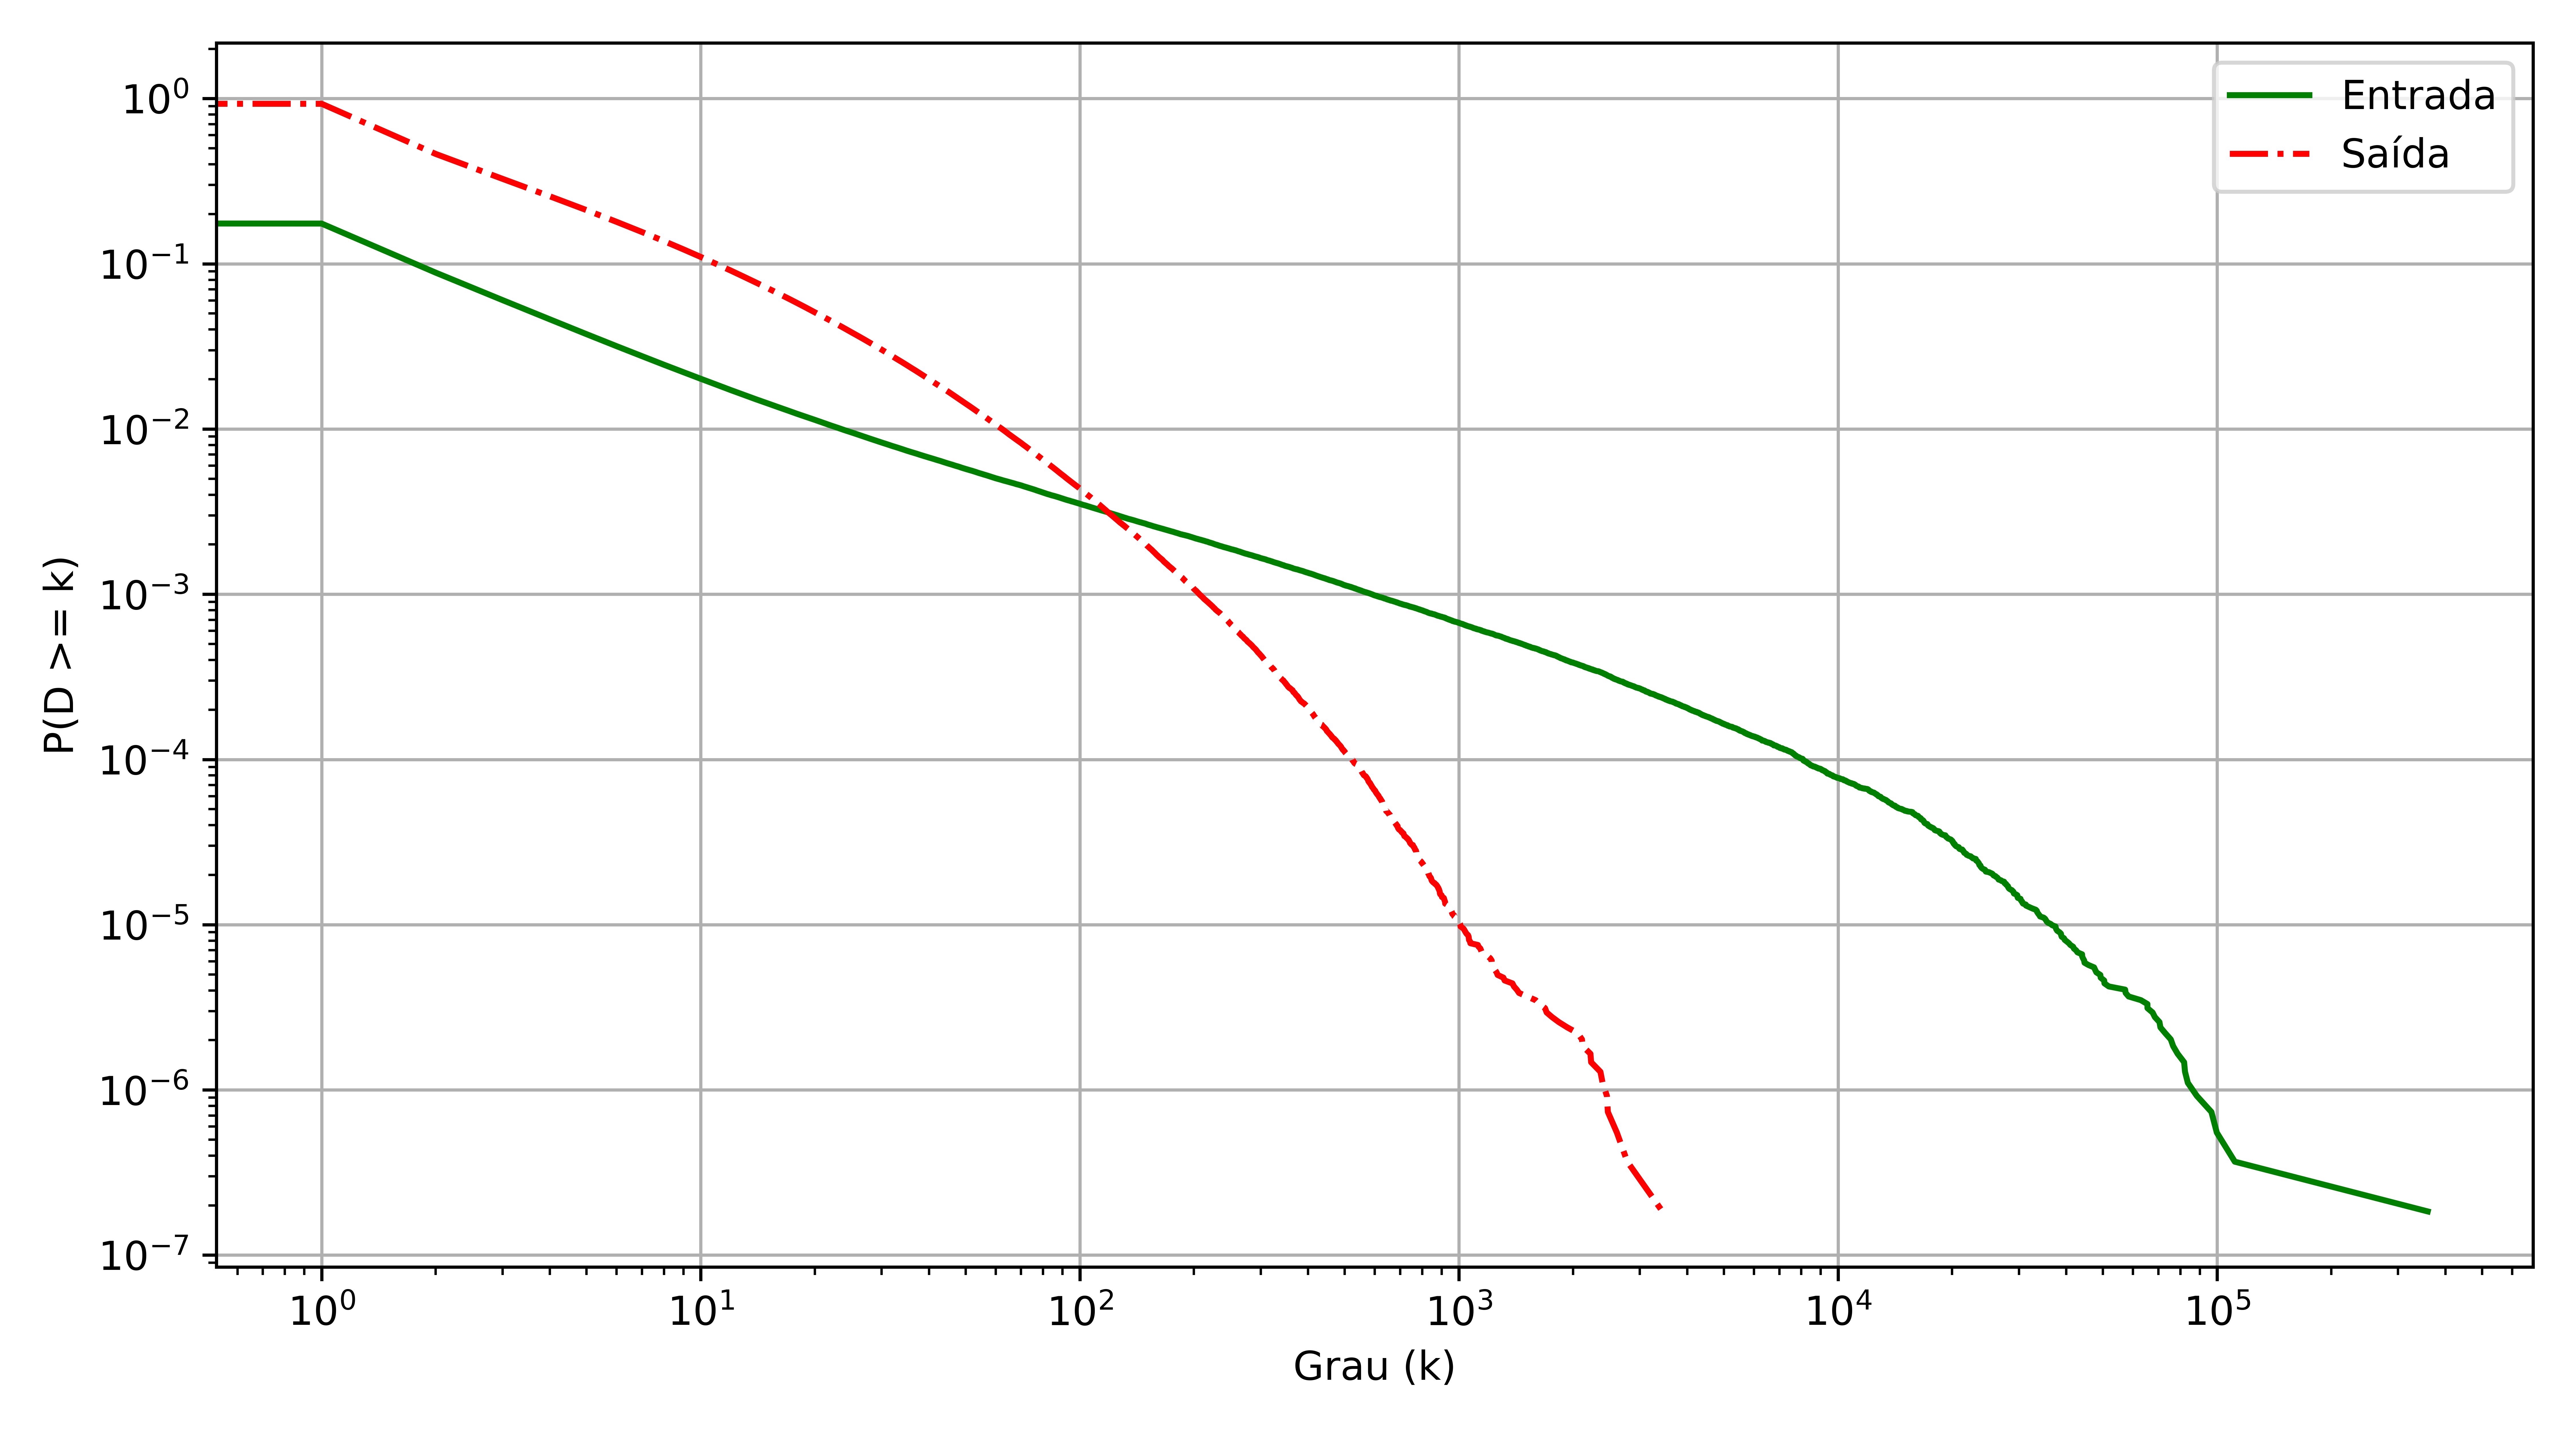
\includegraphics[scale=0.65]{images/graph_ccdf.png}
    \caption{Gráfico da \textit{CCDF (complementary cumulative distribution function)}
             dos graus de entrada e saída da rede de usuários.
             O eixo horizontal representa o grau $k$ enquanto o eixo vertical
             demonstra a probabilidade de um vertice ter grau pelo menos $k$.}
    \label{fig:graph_ccdf}
    \end{center}
}
\end{center}
\end{figure}

\begin{figure}[h]
\begin{center} {
    \begin{center}
    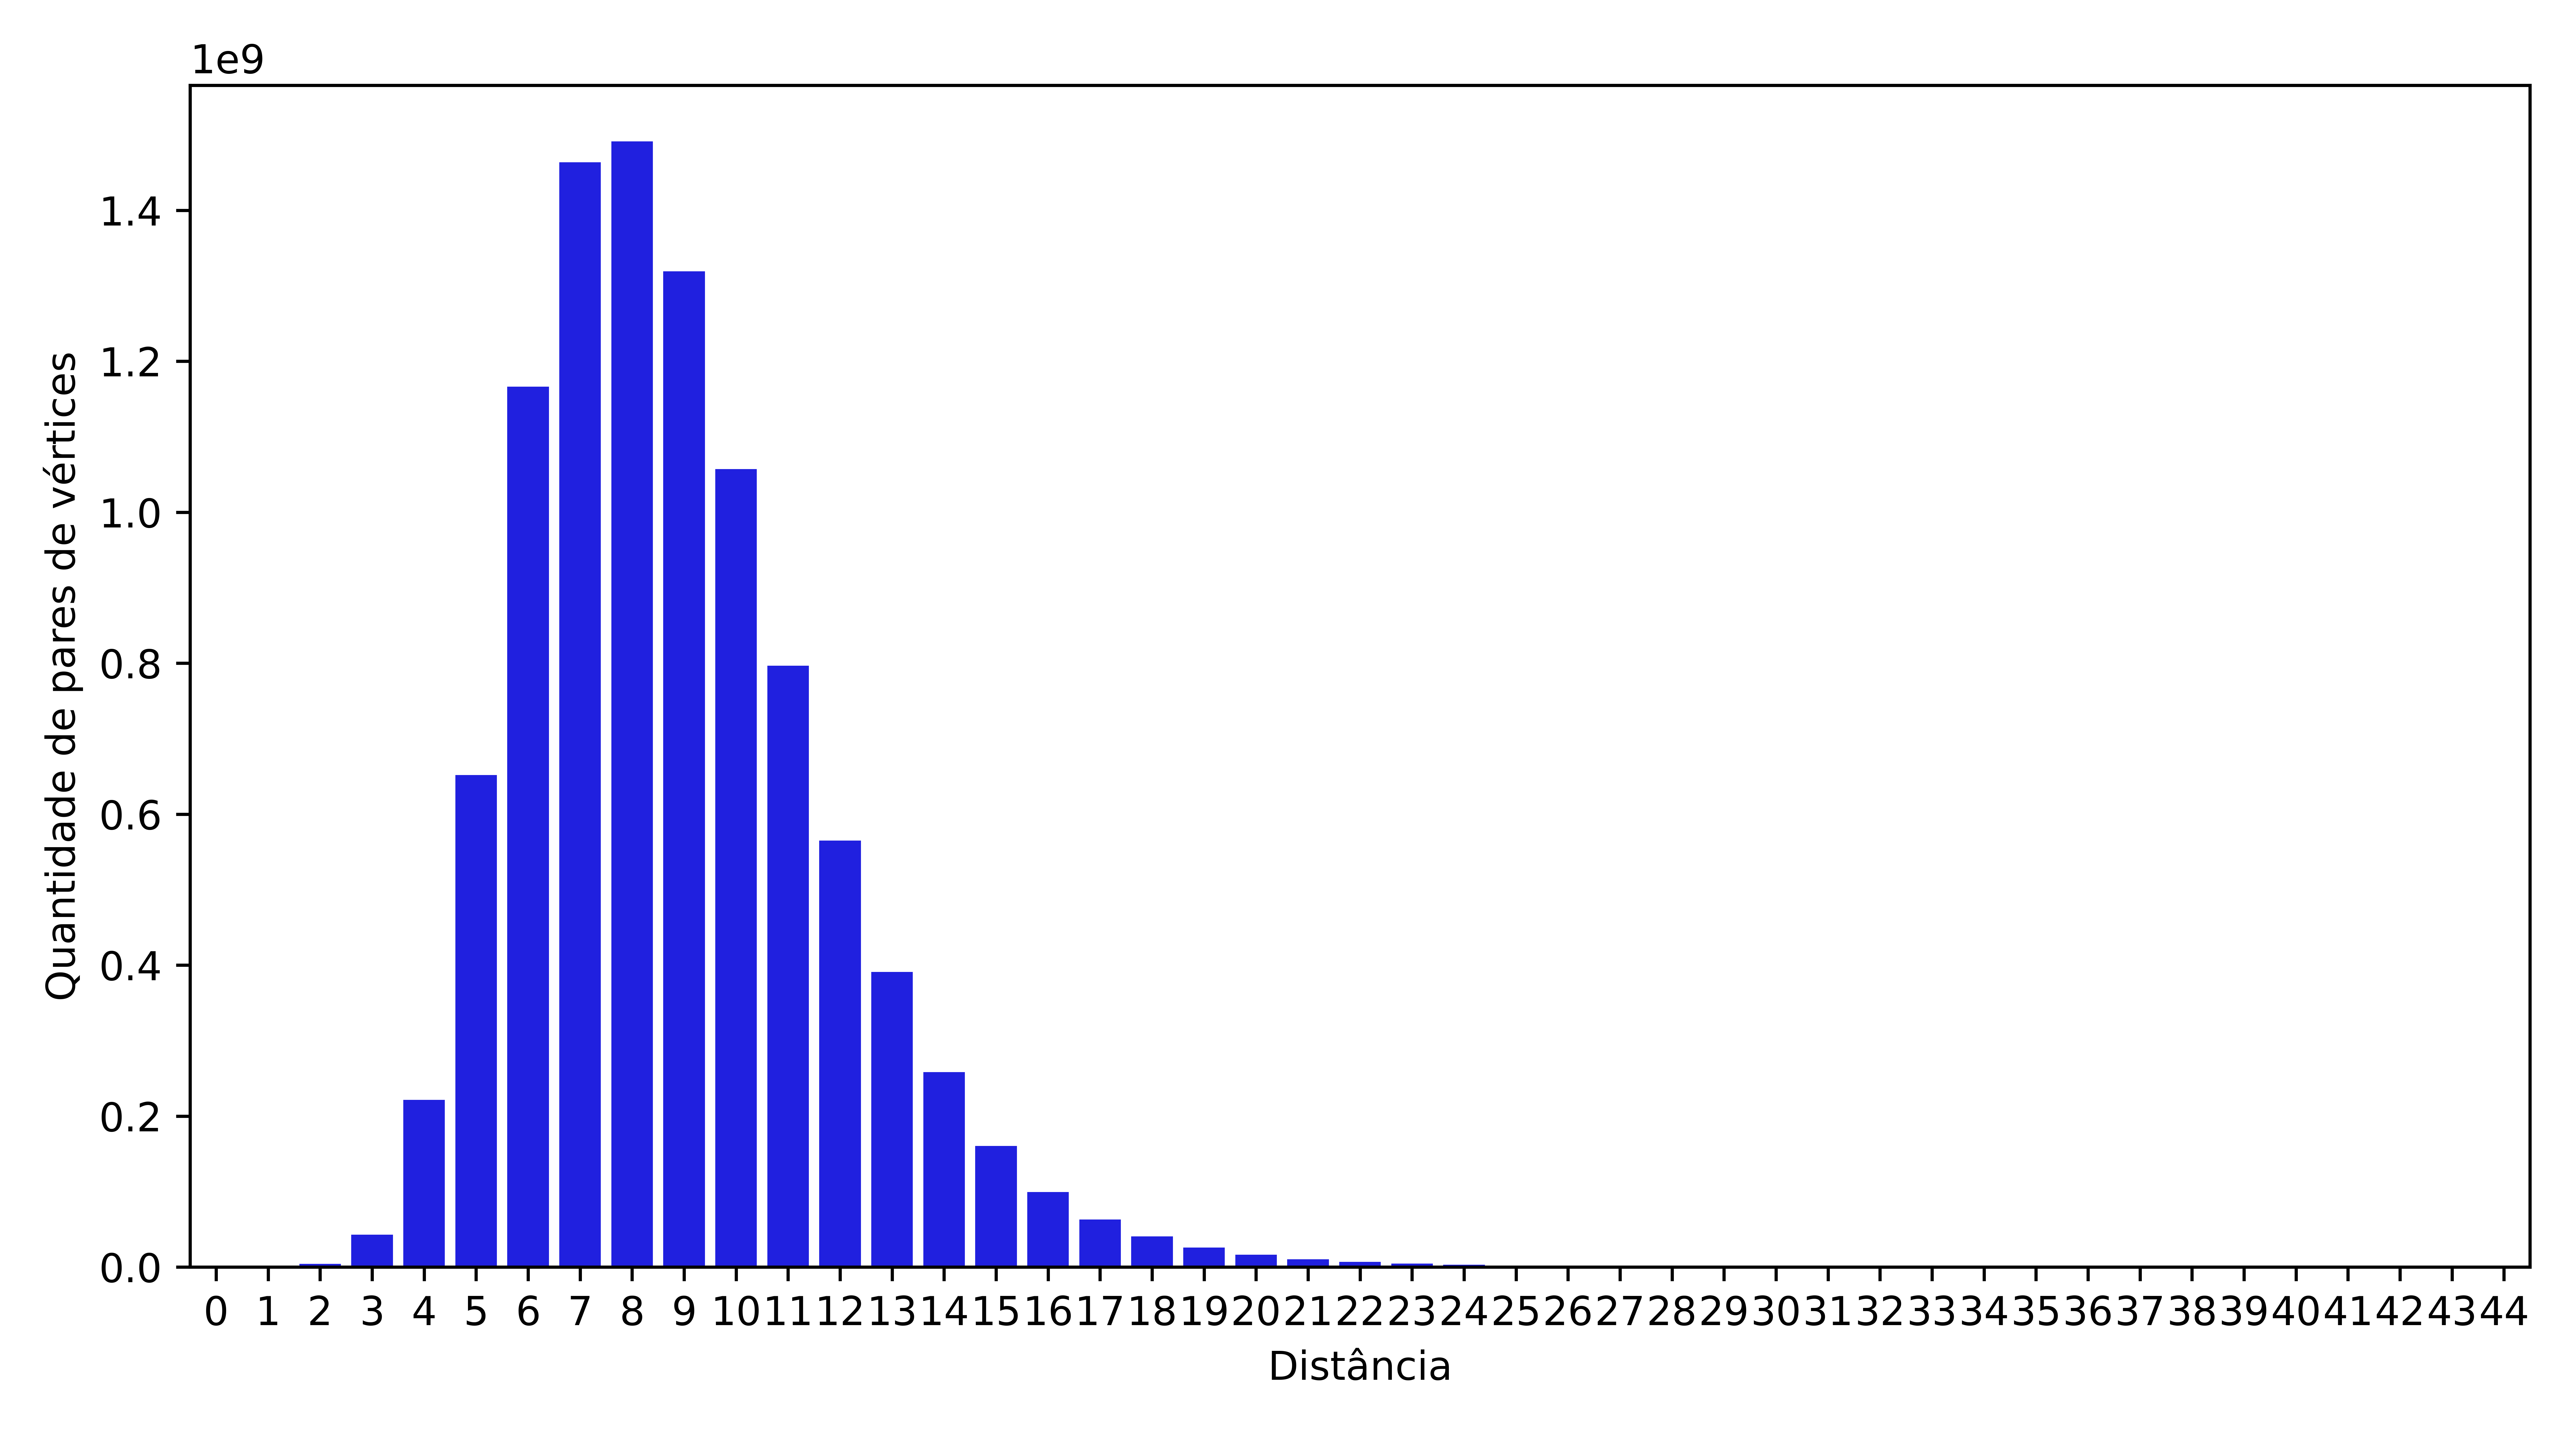
\includegraphics[scale=0.65]{images/graph_distance.png}
    \caption{Distância entre pares de nós da rede de usuários.}
    \label{fig:graph_distance}
    \end{center}
}
\end{center}
\end{figure}

Uma vez finalizada a etapa de coleta dos dados, o processo de anotação e a
formação da rede de usuários, se prosseguiu para a etapa do classificador de
sentimento textuais.
Esses classificadores serão usados como base de comparação para avaliar a
eficiência dos classificadores multi-modais.

Os primeiros classificadores textuais treinados foram os por Naive Bayes e SVM.
Nesse caso, ambos usaram a representação Bag-of-Words.
O vocabulário formado a partir da base coletada é formado por um 127 mil
palavras.
O treinamento do algoritmo de Naive Bayes multinomial foi feito utilizando
validação cruzada por K-partições, no total de 10 partições, sob os dados de
treinamento anotados com supervisão distante. O parâmetro de suavização foi
escolhido por \textit{grid search}, de maneira a maximizar a área sob a curva ROC.
A Figura~\ref{fig:nb_grid} mostra a resposta do modelo para os diferentes fatores
de suavização testados.
O hiperparâmetro selecionado foi o de valor $0,244$, que obteve AUC de $0,862 \pm 0,002$.
Uma vez selecionado o melhor modelo na base de treino, o mesmo foi avaliado com
os dados da base de teste, que foram anotados manualmente.
A Figura~\ref{fig:nb_roc} apresenta a curva ROC dos dados de treino.
Observa-se que o mesmo modelo ao ser aplicado aos dados de teste tem resultado
de $0,801$ de área sob curva ROC.
Vê-se que há uma diferença de performance entre as diferentes bases, que
sobressaí a dispersão observada nas partições do treinamento.
Este aspecto da supervisão distante será discutido no Capítulo~\ref{chapter:conclusion}.
Concluindo a análise do modelo de Naive Bayes, a Figura~\ref{fig:nb_residuo}...

\begin{figure}[h]
\begin{center} {
    \begin{center}
    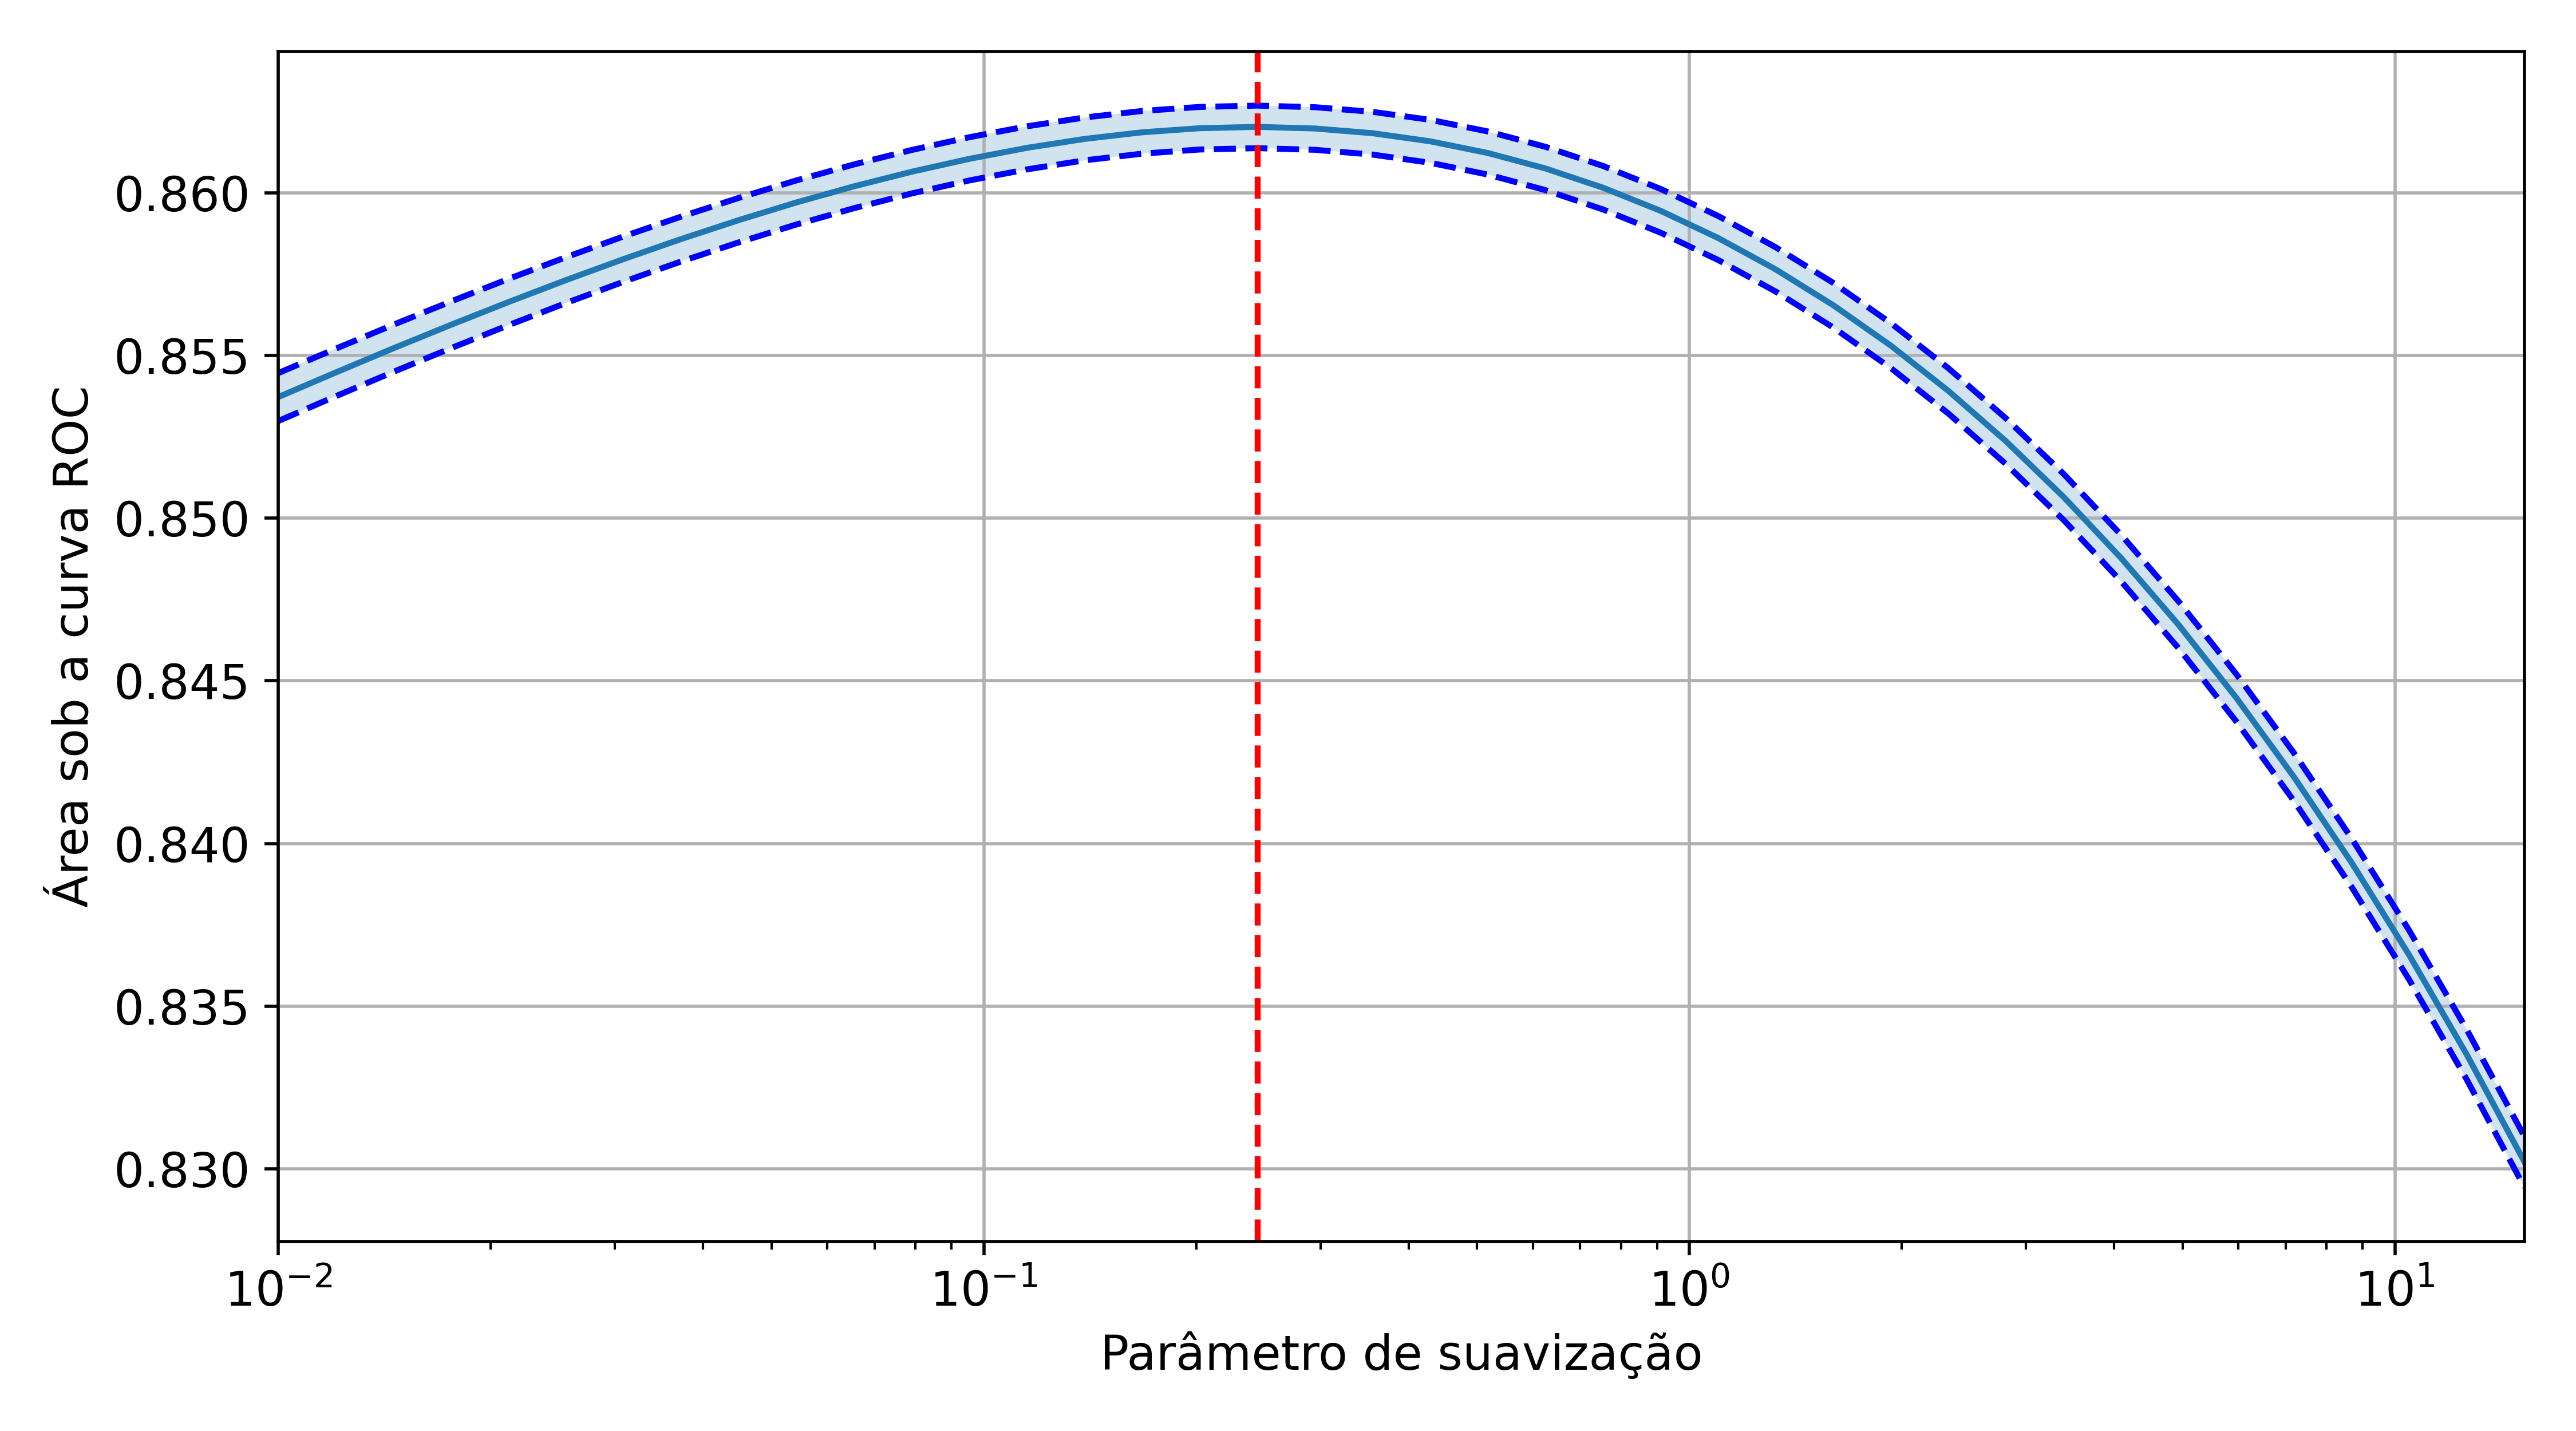
\includegraphics[scale=0.65]{images/nb_grid.png}
    \caption{Resposta do modelo de Naive Bayes a variação do parâmetro de suavização.
             A linha cheia representa a média dos valores das 10 partições
             enquanto a área em azul, limitada pela linha rachurada, representa um desvio padrão.
             A linha vertical vermelha ressalta o paramêtro de maior média.}
    \label{fig:nb_grid}
    \end{center}
}
\end{center}
\end{figure}


\begin{figure}[h]
\begin{center} {
    \begin{center}
    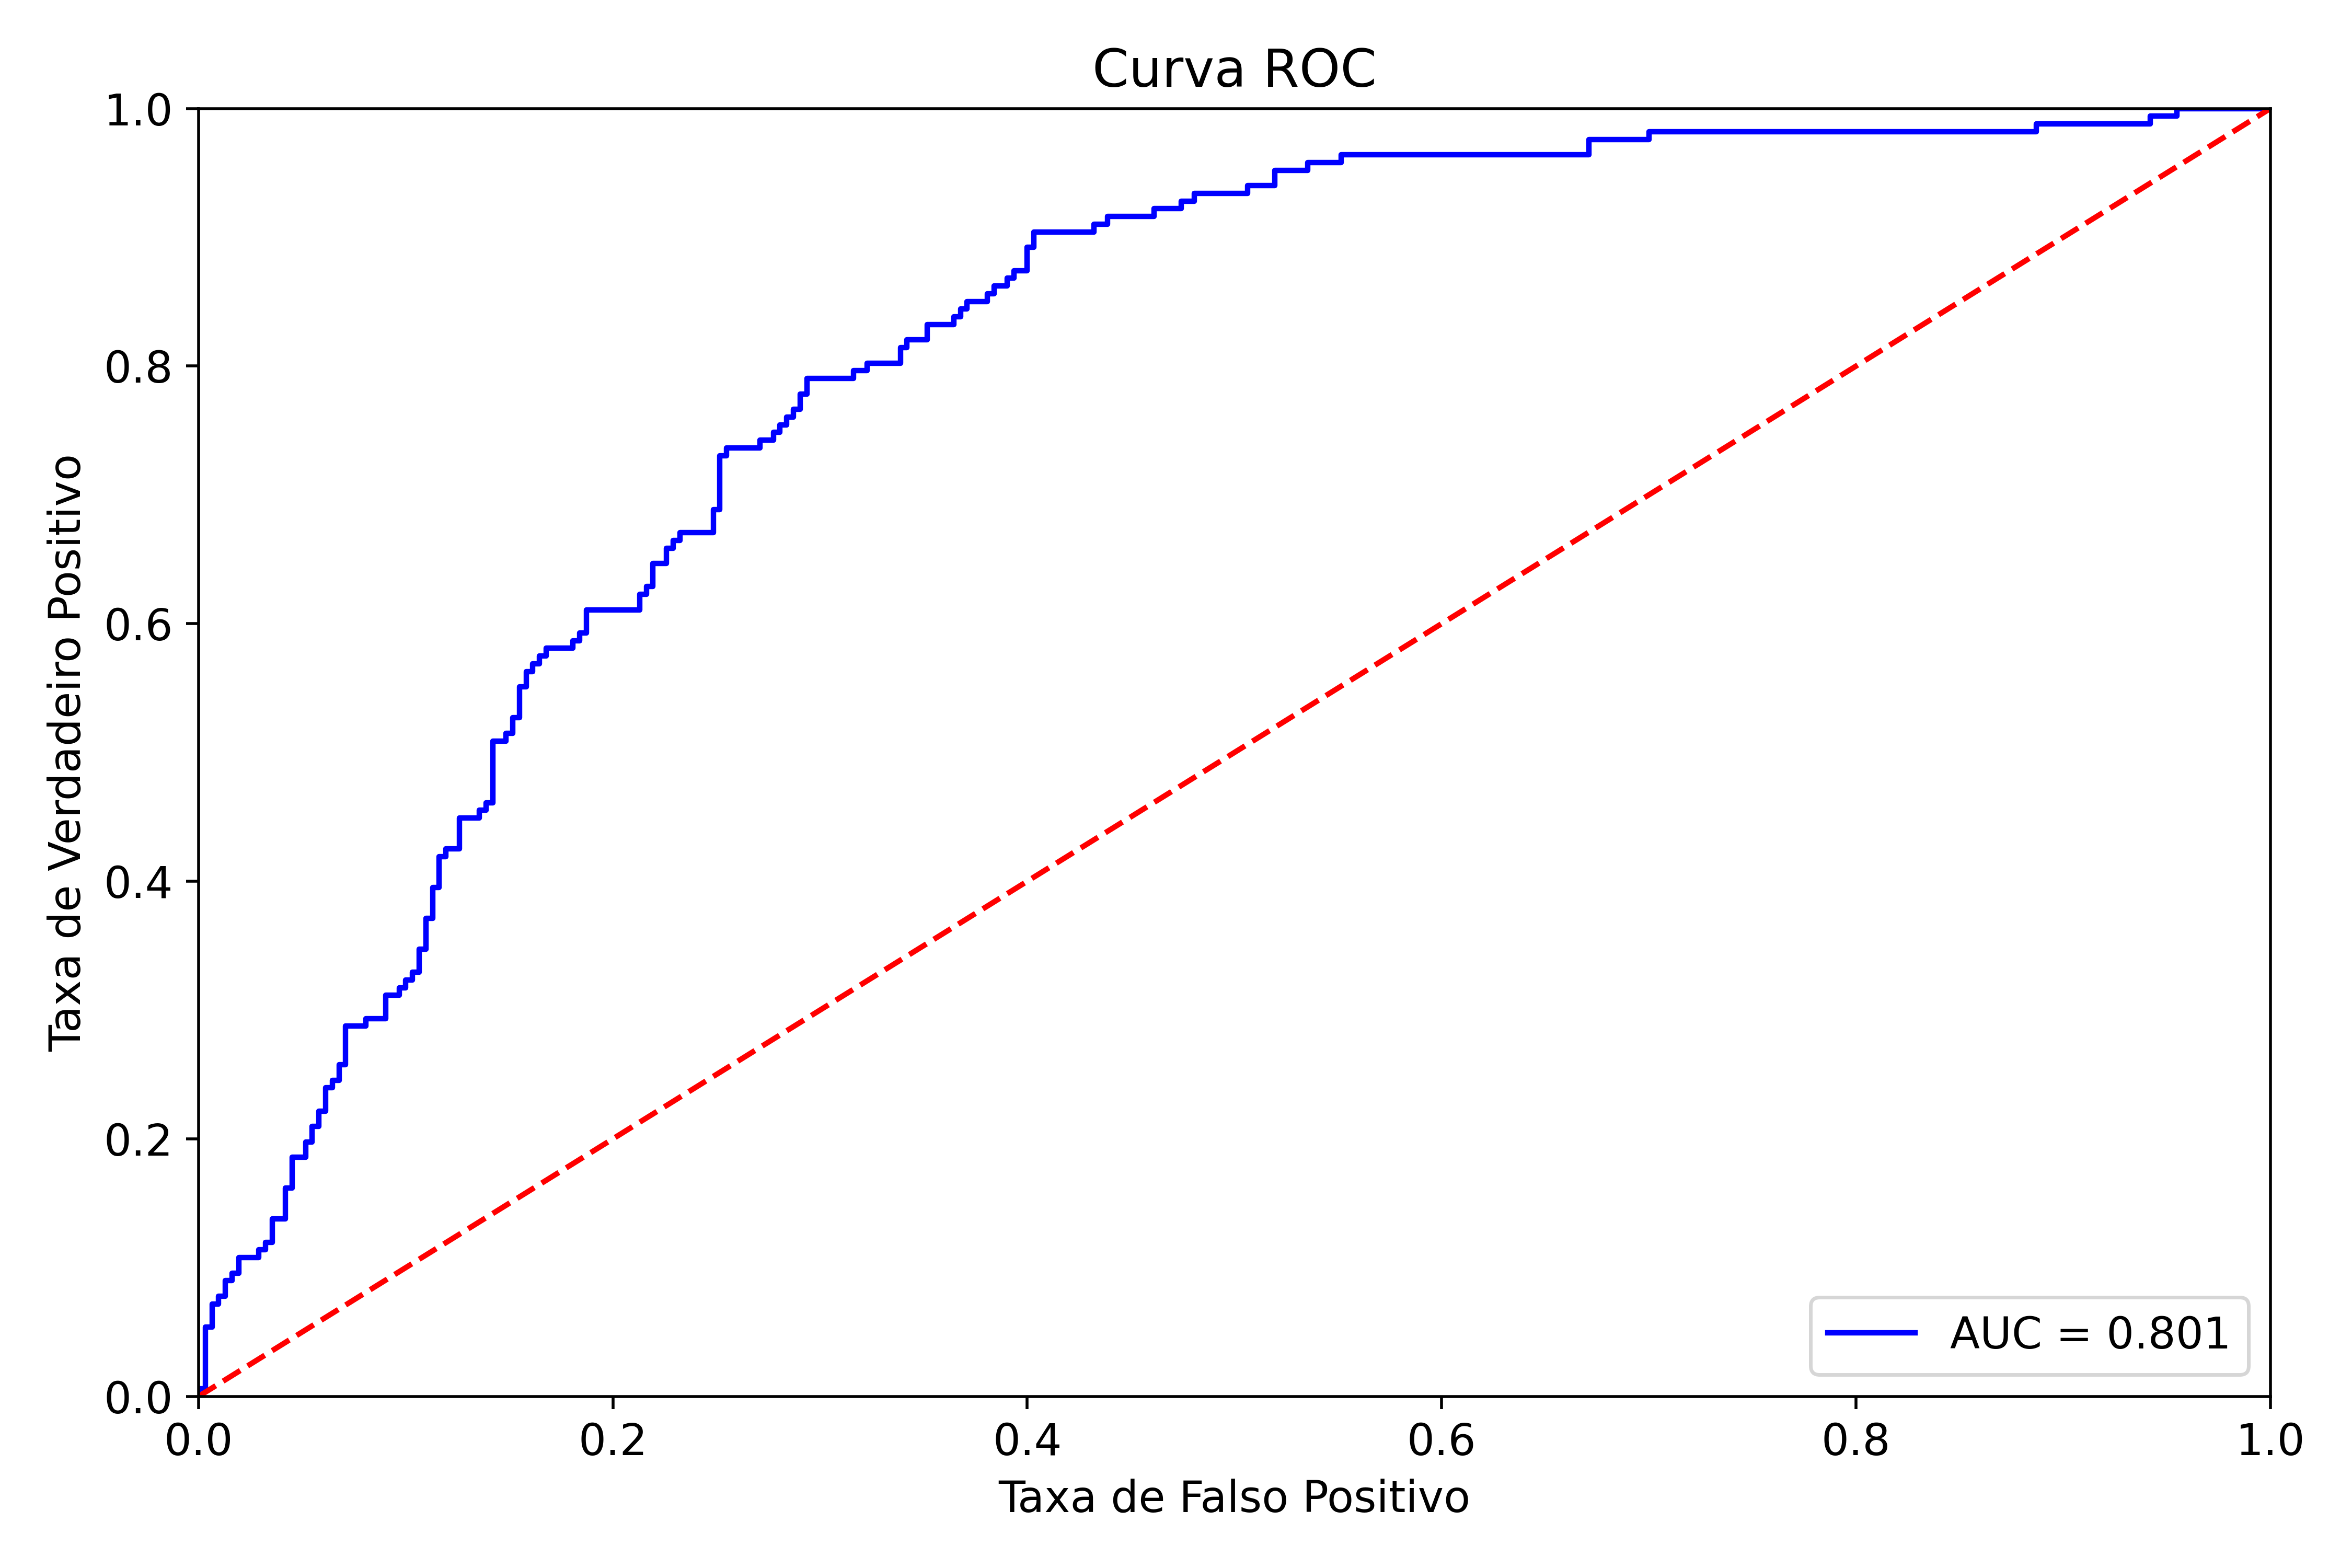
\includegraphics[scale=0.65]{images/nb_roc.png}
    \caption{LOREM IPSUM}
    \label{fig:nb_grid}
    \end{center}
}
\end{center}
\end{figure}
% grafico residuo
